\documentclass[a4paper]{article}
\usepackage[utf8]{inputenc}
\usepackage[spanish, es-tabla, es-noshorthands]{babel}
\usepackage[table,xcdraw]{xcolor}
\usepackage[a4paper, footnotesep = 1cm, width=20cm, top=2.5cm, height=25cm, textwidth=18cm, textheight=25cm]{geometry}
%\geometry{showframe}

\usepackage{tikz}
\usepackage{amsmath}
\usepackage{amsfonts}
\usepackage{amssymb}
\usepackage{float}
\usepackage{graphicx}
\usepackage{caption}
\usepackage{subcaption}
\usepackage{multicol}
\usepackage{multirow}
\setlength{\doublerulesep}{\arrayrulewidth}
\usepackage{booktabs}

\usepackage{hyperref}
\hypersetup{
    colorlinks=true,
    linkcolor=blue,
    filecolor=magenta,      
    urlcolor=blue,
    citecolor=blue,    
}

\newcommand{\quotes}[1]{``#1''}
\usepackage{array}
\newcolumntype{C}[1]{>{\centering\let\newline\\\arraybackslash\hspace{0pt}}m{#1}}
\usepackage[american]{circuitikz}
\usetikzlibrary{calc}
\usepackage{fancyhdr}
\usepackage{units} 

\graphicspath{{../Calculos-Potencia/}{../Caracteristicas/}{../Consideraciones/}{../Gain-Stage/}{../Input-Stage/}{../Output-Stage/}{../Simulaciones/}{../Alimentacion/}{../Conclusiones/}}

\pagestyle{fancy}
\fancyhf{}
\lhead{22.12 Electrónica II}
\rhead{Mechoulam, Lambertucci, Rodriguez, Londero, Scala}
\rfoot{Página \thepage}

\begin{document}
	
\subsubsection{Consideraciones de diseño}
Se diseño una fuente de tensión regulada con limitación de corriente enfocados en alcanzar la menor disipación de potencia posible. 
Los requerimientos de la misma son los siguientes:
\\ 
\textbf{Corriente de salida:}
\begin{equation}
	I = [0mA, 200mA]
\end{equation}
\\
\textbf{Tensión de salida:}
\begin{equation}
V_{o} = 5 \pm 3\%
\end{equation}

Otro punto de interés es el de minimizar la cantidad de componentes utilizados. Por lo tanto se decidió utilizar una protección del tipo lineal en vez de foldback.

A continuación se explicara brevemente el primer diseño propuesto para luego dar lugar a una explicación más detallada sobre un versión optimizada de la fuente.

\subsubsection{Primer diseño propuesto}
El primer diseño que se propuso fue el siguiente:
\begin{figure}[H]
	\centering
	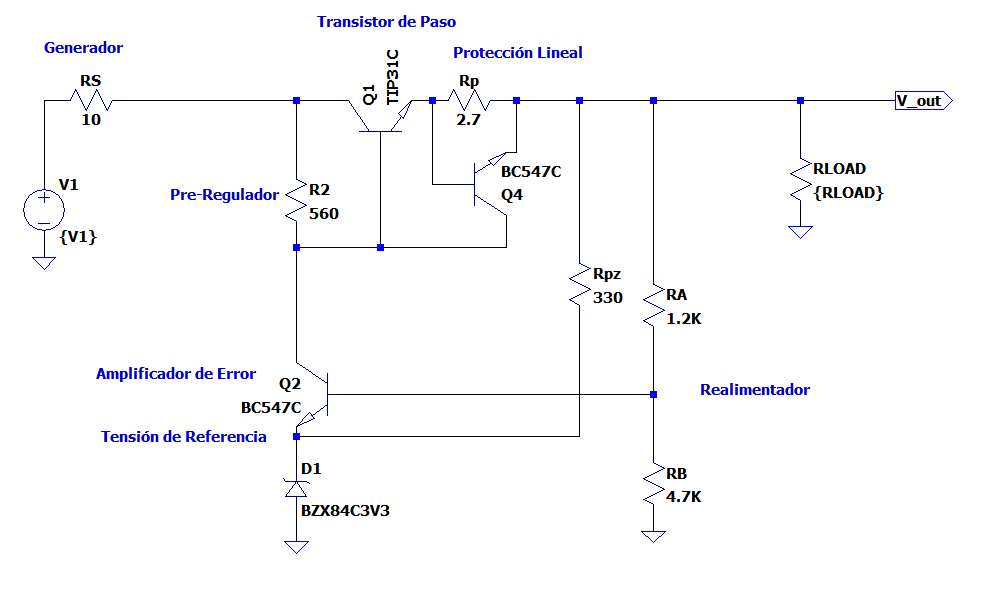
\includegraphics[width=0.7\linewidth]{ImagenesEjercicio1/ImagenCircuitoFV}
	\caption{Fuente de tensión regulada con limitación de corriente}
	\label{fig:imagencircuito}
\end{figure}

La \textbf{tensión de referencia} le permite al amplificador de error saber cuando debe compensar su salida ante variaciones en la tensión de salida. 
En este caso se decidió que la tensión de referencia fuese de $V_{ref} = 4V$ dado que era posible utilizar una combinación de valores comerciales de resistencias tal que:
\begin{equation}
	V_{ref}  = V_{o} \cdot \frac{R_B}{R_A + R_B}
\end{equation} 
Dado que 
\begin{equation}
	V_{ref} \approx 5 \cdot 0.7966
\end{equation}
\begin{equation}
	V{ref} = 4 \pm 0.5 \%
\end{equation}

Para diseñar el Pre-Regulador se tuvo en cuenta la ganancia de corriente del transistor de paso \textbf{Q1}.
\begin{figure}[H]
	\centering
	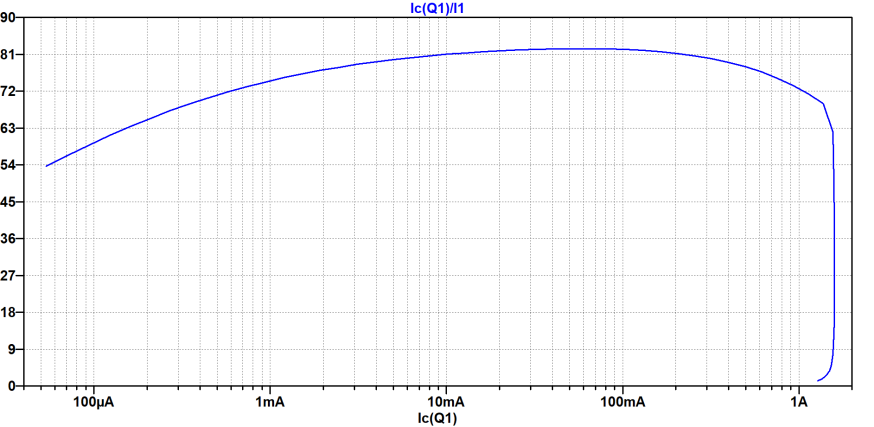
\includegraphics[width=0.7\linewidth]{ImagenesEjercicio1/BetaTPasoFV}
	\caption{Curva de la ganancia de corriente $\beta$. $V_{ce}=2.52$}
	\label{fig:betatpasofv}
\end{figure}
Cuando la carga sea mínima el transistor de paso experimentara el mayor flujo de corriente. En este caso ese valor es de unos 205 $mA$ aproximadamente. Remitiéndonos al gráfico vemos que la ganancia de corriente se ubica por encima de 80. 
Por lo tanto podemos obtener la siguiente expresión para el calculo de $R_2$. Debemos tener en cuenta que esto ocurre cuando el transistor \textbf{Q2} se encuentra en corte.

\begin{equation}
R_{2} = \frac{V_{gen}-R_{g}\cdot I_{o_{max}} - (V_o - V_{be_{Q3}} - V_{be_{Q1}}  )}{I_o} \cdot \beta
\end{equation}
\begin{equation}
R_{2} = \frac{10 - 10 \Omega \cdot 205mA - (5V - 0.580 -0.7)  }{200mA} \cdot 80
\end{equation}
\begin{equation}
R_{2} = 668 \Omega
\end{equation}
El valor de resistencia obtenido es un valor \textbf{no} comercial. Podríamos ir por el valor más próximo, 680 $\Omega$ pero este valor no cumple con las especificaciones. Por lo tanto optamos por el valor comercial menor más próximo 560 $\Omega$
\subsubsection{Circuito de Protección}
La resistencia de protección se calculo teniendo en cuenta que la corriente de emisor del transistor de paso incluía la corriente necesaria para la polarización del diodo Zener. 
\begin{equation}
	R_p = \frac{V_{be_{Q3}}}{I_{emisor}}
\end{equation}

El \textbf{elemento de referencia} en este caso se escogió como la combinación de la tensión de Zener y $V_{be_{ON}}$
\begin{equation}
	V_{ref} = V_{zener} + V_{be_{ON}}
\end{equation}

Para poder obtener la recta de carga podemos optar por usar la directiva de spice \textit{.step param} o bien podemos simular una carga variable mediante el uso de una fuente de corriente. El ultimo método nos ofrece una mayor velocidad de simulación y gráficos de mayor calidad.

\begin{figure}[H]
	\centering
	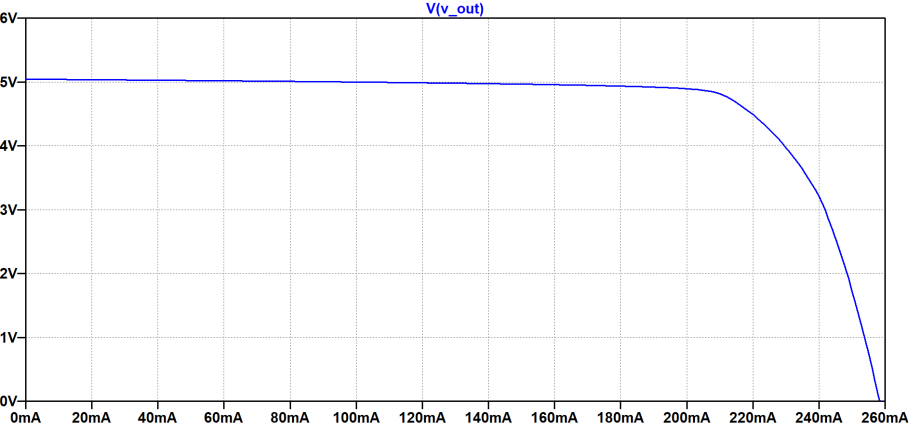
\includegraphics[width=0.7\linewidth]{ImagenesEjercicio1/CaracteristicaDeSalidaConGrillaFV}
	\caption{Característica de Salida Diseño 1}
	\label{fig:caracteristicadesalidacongrillafv}
\end{figure}

Este gráfico nos indica que el circuito ofrece una buena regulación de tensión dentro del rango de corriente requerido. Sin embargo notamos algo inesperado, a partir de los $200mA$ no tenemos una caída abrupta de la tensión sino más bien una caída suave hacia 0. Estudiaremos esto en más detalle en la próxima sección.

\subsection{Segunda iteración de diseño}
Utilizar la menor cantidad de componentes ofrece varios beneficios como por ejemplo, menos efectos de las tolerancias, mayor aprovechamiento del espacio y mayor sencillez de diseño.
A continuación presentamos el diseño resultante:
\begin{figure}[H]
	\centering
	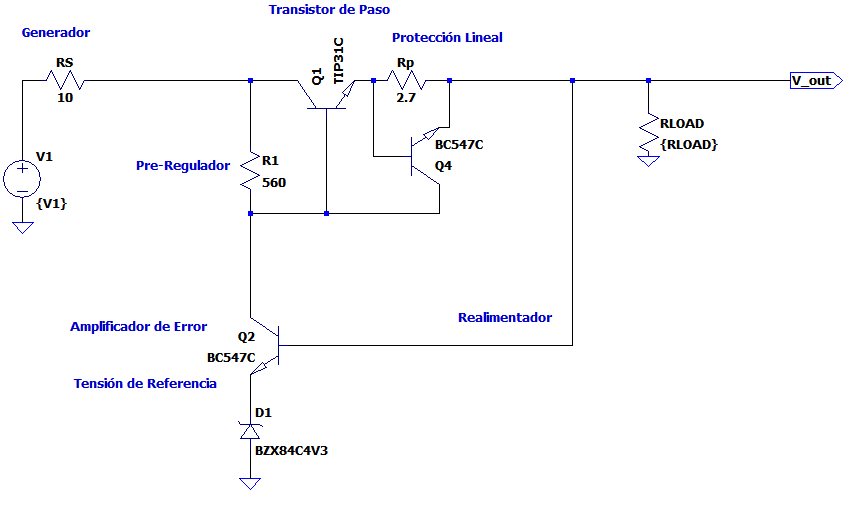
\includegraphics[width=0.7\linewidth]{ImagenesEjercicio1/ImagenCircuitoFL}
	\caption{}
	\label{fig:imagencircuitofl}
\end{figure}
En esta oportunidad se realizaron 2 cambios importantes. En primer lugar se decidio cambiar el diodo Zener utilizado, en esta ocasión $V_z$ = $4.3V$ para que junto con la tensión $V_{be}$.
Ahora el nuevo voltaje de referencia es:
\begin{equation}
	V_{ref} = V_{be_{ON}} + V_{zener}
	V_{ref} = 5V
\end{equation}
Este nuevo resultado implica que ya no es necesario utilizar un realimentador del tipo divisor resistivo ¡Podemos usar un cable! Eso implica el ahorro de 2 resistencias y el consumo de potencia (aunque pequeño) que conllevan.


TOBIAS COMPLETA ACA !!

No obstante, es posible hacerle una mejora más y mucho más importante en términos de consumo. Las siguientes observaciones nos abrirán camino hacia esta nueva mejora.

Comenzamos por estudiar la resistencia de polarización $R_{pz}$ que deberíamos colocar para el correcto funcionamiento del diodo.
\begin{equation}
	R_{pz} = \frac{5\Omega-4.3\Omega}{7mA}
\end{equation}


Por lo tanto disipa xx mW.

Pero, ¿Es posible evitar colocarla? La respuesta es afirmativa pero antes debemos modificar


HASTA ACÁ!!

En este caso obtenemos una característica de salida similar a la anteriormente obtenida.




%El Zener sigue polarizado porque 
%Cuando el circuito deja de regular sigue consumiendo potencia en el viejo.
%V max: 
%V min: 



\end{document}